\documentclass[18pt, aspectratio=169]{beamer}
% \documentclass{etp-beamer-fancy}
\usepackage[utf8]{inputenc}
% \usepackage{templates/mytemplate}
\usepackage{templates/beamerthemekit}
\usepackage{graphicx}
\usepackage{microtype}
\usepackage{xcolor}
\usepackage{hyperref}
\usepackage{siunitx}
\usepackage{upgreek}
\usepackage{hepnames}
\usepackage{appendixnumberbeamer}
\usepackage{booktabs}
\NewDocumentCommand\angrange{O{} m m}{\SIrange[parse-numbers=false,#1]{\ang[parse-numbers=true]{#2}}{\ang[parse-numbers=true]{#3}}{}}
\usepackage{subcaption}
% \usepackage{enumitem}

\title{MVA Track Quality Estimation for the Belle II Experiment}
\subtitle{Tracking Meeting}
\author[Michael Eliachevitch
(\href{mailto:michael.eliachevitch@kit.edu}{michael.eliachevitch@kit.edu})]{Michael Eliachevitch(\href{mailto:michael.eliachevitch@kit.edu}{michael.eliachevitch@kit.edu})}
\titleimage{tracks_wide}
\titlelogo{belle2-logo}
\institute[ETP -- KIT]{Institut für Experimentelle Teilchenphysik (ETP) -- KIT}
\date{26 April 2019}

\newcommand{\kitemph}[1]{\textcolor{kit-green100}{\bf{#1}}}

\begin{document}
\maketitle
\begin{frame}
  \frametitle{Track Quality Indicator}
  \begin{itemize}
  \item Goal: Enable physics analysts to \kitemph{choose working point} on the efficiency vs.
    purity receiver operating curve (ROC)
  \item assign a \kitemph{quality indicator (QI)} to the final tracks
  \item include low-level \kitemph{tracking information} in addition to already existing information
    from the fit (e.g.\ $\chi^2$),
  \item Solution: Train an multivariate (MVA) classifier $=$ \kitemph{track quality estimator}
  \end{itemize}
\end{frame}
\begin{frame}
  \frametitle{Features for Training the Quality Estimator}
    \begin{itemize}
    \item training target: MC truth to discriminate fake (and clone) from correct tracks in training
    \item input variables: use all information available during the reconstruction
    \item intermediate quality estimators: \kitemph{CDC QE, VXDTF QE}
      \begin{itemize}
      \item many features only available to the tracking algorithms in the subdetectors, e.g.
      \item CDC: drift lengths, ADC signals, \ldots
      \item SVD: charge, energy loss, triplet fit \ldots
      \end{itemize}
    \item hit patterns and hit weights from the \kitemph{track fit}
    \item momentum and positional information (\kitemph{four-vectors})
    \item timing information
    \item \kitemph{merger information}: $\chi^2$ and differences in track parameters
    \item \kitemph{event-level} variables: bias?
    \end{itemize}
\end{frame}

\begin{frame} 
  \frametitle{Example Feature Distributions}
  \begin{columns}[t]
    \begin{column}{.5\textwidth}
      \center
      From CDC tracking: e.g.\ drift lengths
      \includegraphics[width=\textwidth]{figures/cdc-qi-new/drift_length_sum.pdf}
    \end{column}
    \begin{column}{.5\textwidth}
      \center
      From fit: e.g.\ track-parameters
    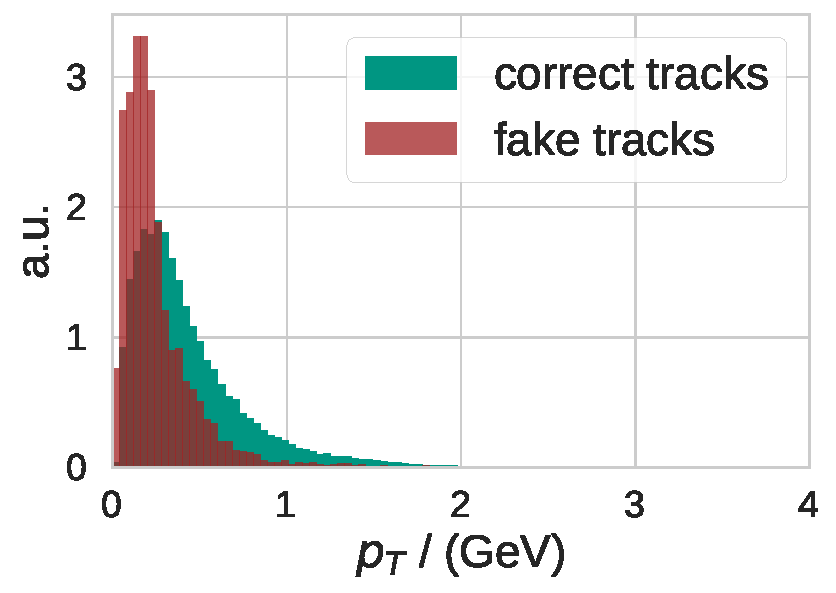
\includegraphics[width=\textwidth]{figures/combined-qi/pt_distributions.pdf}
    \end{column}
  \end{columns}
  \begin{itemize}
  \item these are not the most important ones, just examples
  \item heavily correlated with other variables: FastBDT can learn that
  \end{itemize}
\end{frame}

\begin{frame}
  \frametitle{Training and Validation}
  \begin{columns}
    \begin{column}{.6\textwidth}
      \begin{itemize}
  \item use single steering file with
    \href{https://github.com/nils-braun/b2luigi}{\textcolor{kit-blue100}{b2luigi}}
    \begin{itemize}
    \item combined training and validation of all three classifiers: CDC QE, VXDTF QE and Combined Track QE
    \item easy to iterate over different parameter combinations (e.g.\ grid search)
    \end{itemize}
  \item \num{5000} events ($\sim$ \num{50000} tracks) for each training and separate dataset for
    validation
  \item currently used background: \texttt{15th\_overlay\_phase3\_Feb2018}
  \end{itemize}
  \end{column}
  \begin{column}{.4\textwidth}
    \centering
    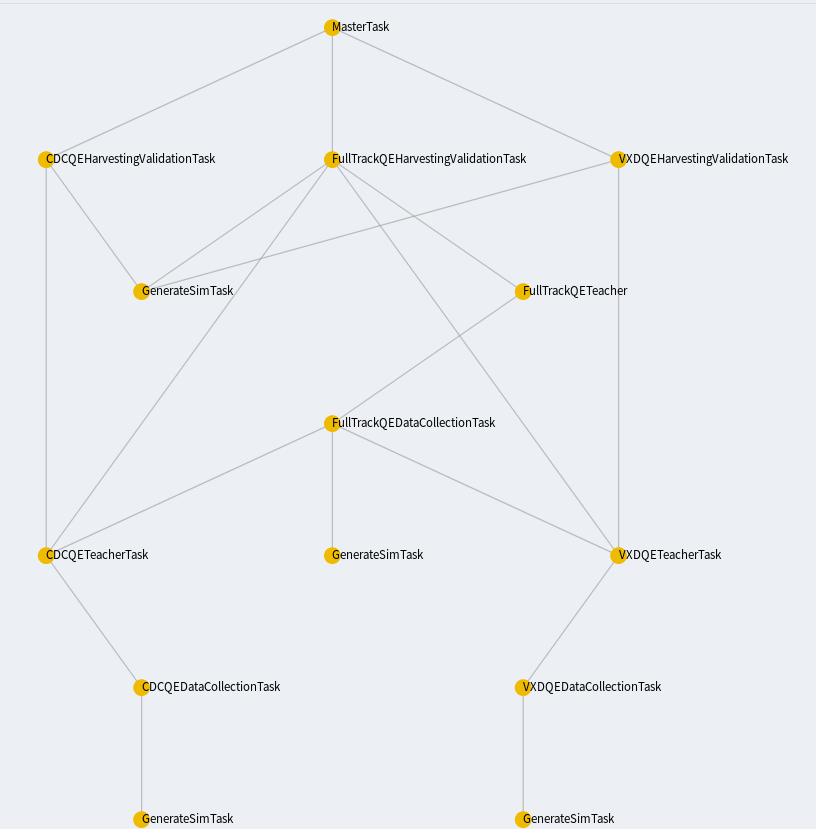
\includegraphics[width=\textwidth]{figures/luigi_task_graph.png}
  \end{column}
\end{columns}    
\end{frame}

\begin{frame}
  \frametitle{CDC Quality Estimator Performance}
  \begin{columns}
    \begin{column}{.33\textwidth}
      \centering
      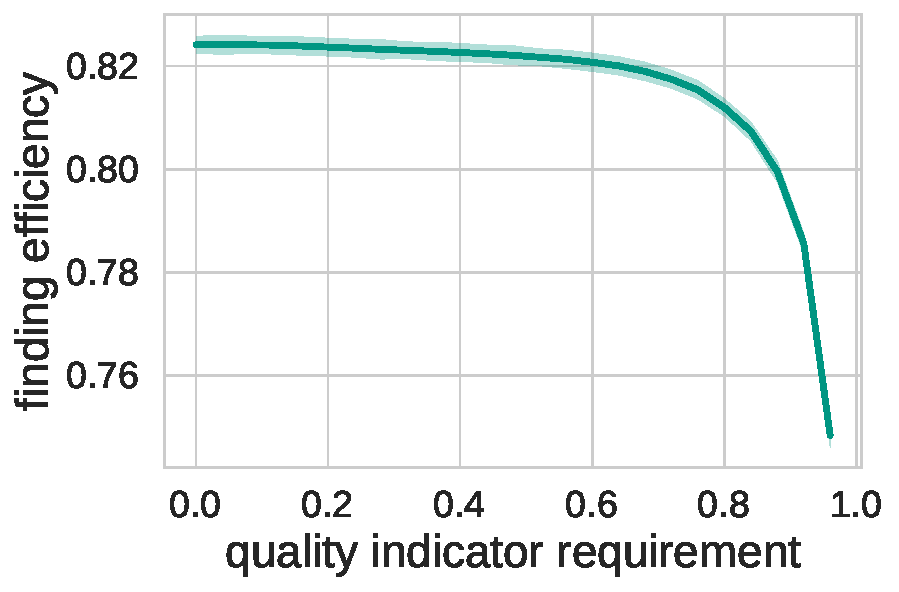
\includegraphics[width=\textwidth]{figures/cdc-qi-new/findeff.pdf}\\
    \end{column}
    \begin{column}{.33\textwidth}
      \centering
            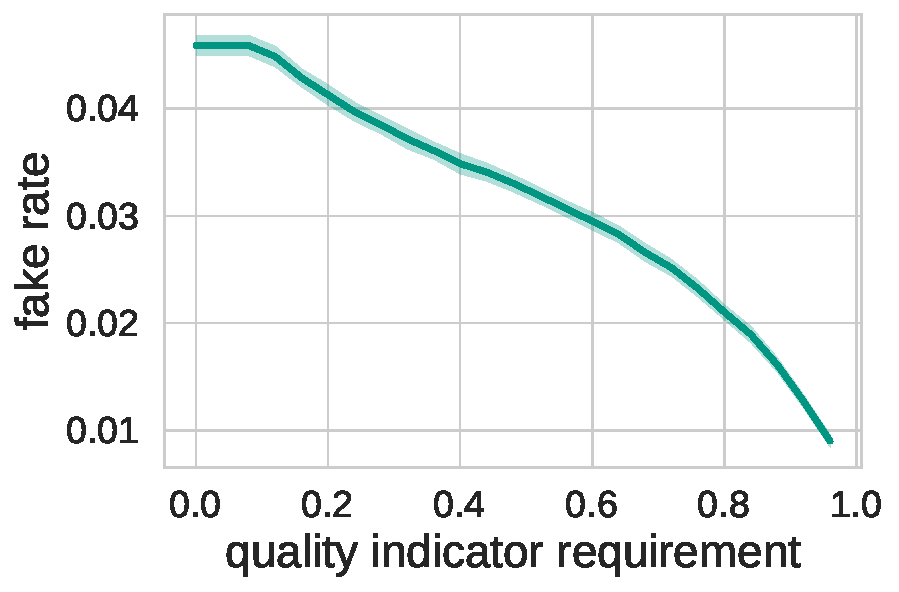
\includegraphics[width=\textwidth]{figures/cdc-qi-new/fake_rate.pdf}\\
    \end{column}
    \begin{column}{.33\textwidth}
      \centering
      \includegraphics[width=\textwidth]{figures/cdc-qi-new/clone_rate.pdf}
    \end{column}
  \end{columns}
  \begin{columns}
    \begin{column}{.4\textwidth}
      \centering
      ROC
      \includegraphics[width=\textwidth]{figures/cdc-qi-new/roc_curve.pdf}
    \end{column}
    \begin{column}{.6\textwidth}
      \begin{itemize}
      \item CDC-only tracking with background
      \item normalized to tracks findable in the CDC
      \item currently trained with clones as background $\rightarrow$~study?
      \end{itemize}
    \end{column}
  \end{columns}
\end{frame}

\begin{frame}
  \frametitle{VXDTF2 Quality Estimator Performance}
  \begin{columns}
    \begin{column}{.33\textwidth}
      \centering
      \includegraphics[width=\textwidth]{figures/vxd-qi/findeff.pdf}\\
    \end{column}
    \begin{column}{.33\textwidth}
      \centering
            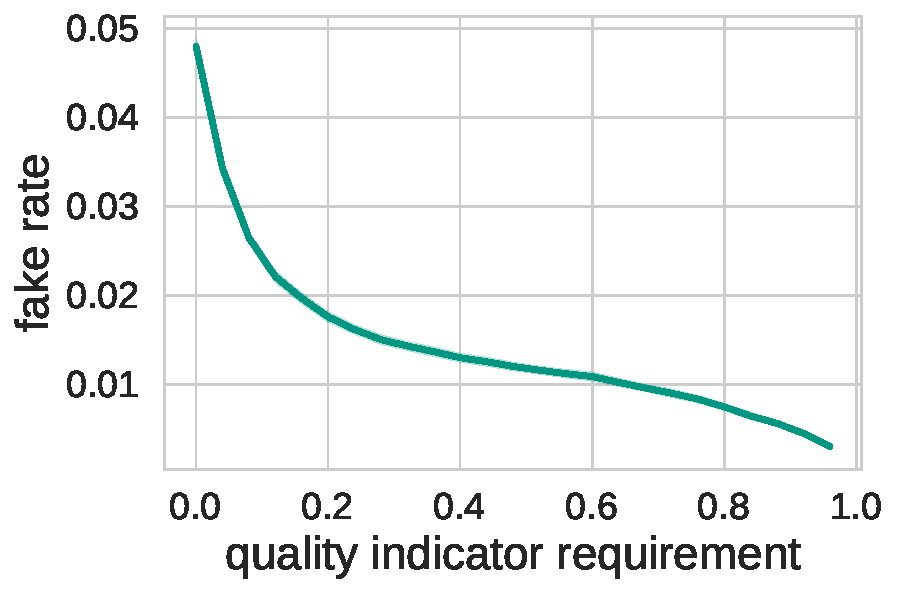
\includegraphics[width=\textwidth]{figures/vxd-qi/fake_rate.pdf}\\
    \end{column}
    \begin{column}{.33\textwidth}
      \centering
      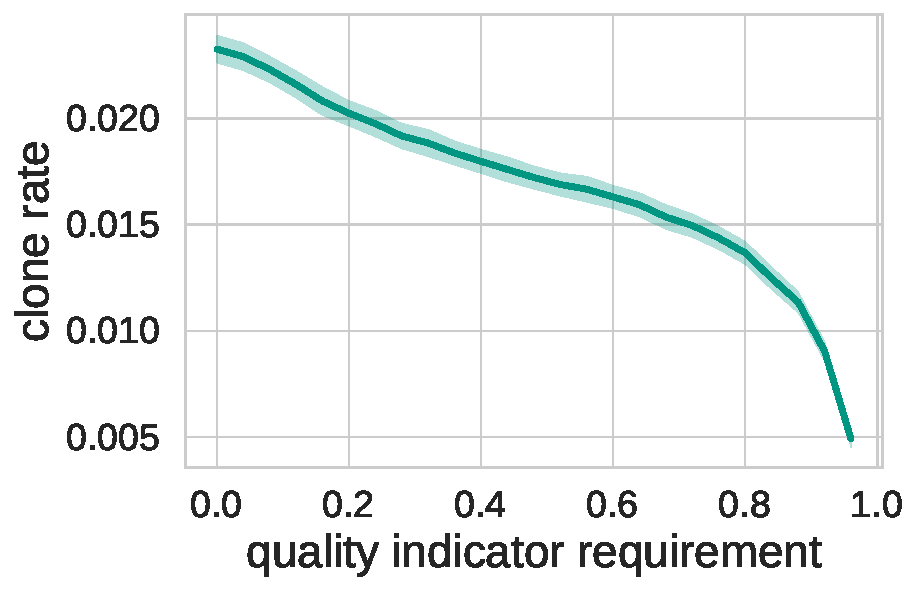
\includegraphics[width=\textwidth]{figures/vxd-qi/clone_rate.pdf}
    \end{column}
  \end{columns}
  \begin{columns}
    \begin{column}{.4\textwidth}
      \centering
      ROC
      \includegraphics[width=\textwidth]{figures/vxd-qi/roc_curve.pdf}
    \end{column}
    \begin{column}{.6\textwidth}
      \begin{itemize}
      \item VXD-only tracking with background
      \item normalized to tracks findable in the VXD
      \item trained with fakes as background class only
      \item in contrast to CDC QE, fake rate falls very steeply at low QI
      \end{itemize}
    \end{column}
  \end{columns}
\end{frame}

\begin{frame}
  \frametitle{Combined Quality Estimation}
  \begin{columns}
    \begin{column}{.33\textwidth}
      \centering
      \includegraphics[width=\textwidth]{figures/combined-qi/fullqi_findeff.pdf}\\
    \end{column}
    \begin{column}{.33\textwidth}
      \centering
      \includegraphics[width=\textwidth]{figures/combined-qi/fullqi_fake_rate.pdf}\\
    \end{column}
    \begin{column}{.33\textwidth}
      \centering
      \includegraphics[width=\textwidth]{figures/combined-qi/fullqi_clone_rate.pdf}
    \end{column}
  \end{columns}
  \begin{columns}
    \begin{column}{.4\textwidth}
      \centering
      ROC
      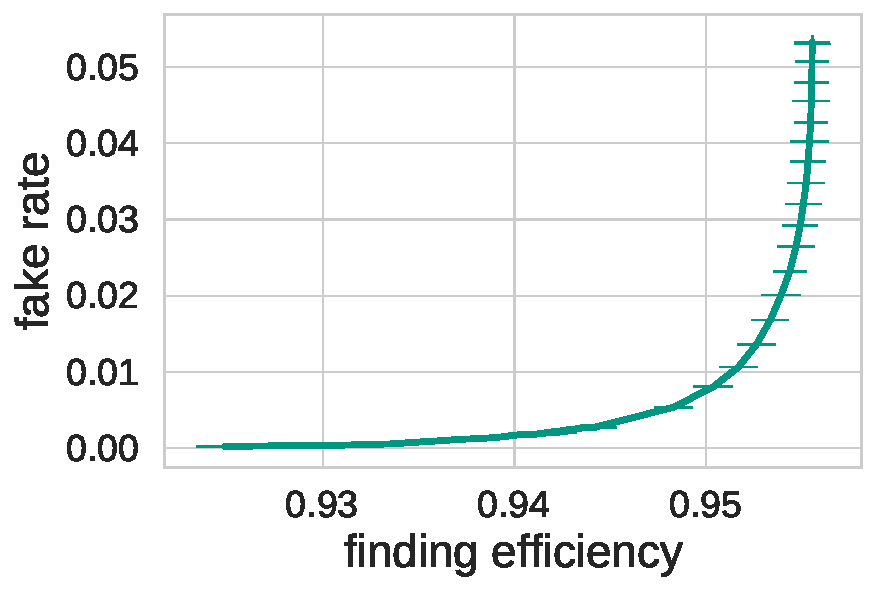
\includegraphics[width=\textwidth]{figures/combined-qi/fullqi_roc_curve.pdf}
    \end{column}
    \begin{column}{.7\textwidth}
      \begin{itemize}
      \item combining features of all track finders yields good fake suppression with only small
        finding efficiency losses
      \item no impact on fitted parameter resolutions in correct PR tracks seen (plots in backup)
      \end{itemize}
    \end{column}
  \end{columns}
\end{frame}

\begin{frame}
  \frametitle{Current Status and ToDo's}
    \begin{itemize}
    \item CDC and VXDTF quality estimators merged, combined quality indicator on branch
      \texttt{feature/BII-2127-General-MVA-QI}
    \item currently finalizing (refactoring) branch, e.g.\ warnings during training
    \item want to compare training with fake-only background in CDC
    \item train without event-level variables?\\
      $\Rightarrow$ easy with luigi
    \item create payloads for CDC QE, VXDQE, combined QE
    \item will create (TUPPR) PR soon so that discussions can happen in the comments
    \end{itemize}
\end{frame}

\appendix
\backupbegin

\begin{frame}
  \centering \huge
  Backup
\end{frame}

\begin{frame}
  \frametitle{MVA Training Parameters}
  \begin{itemize}
  \item train on \num{5000} events ($\sim$\num{50 000} tracks) each for training and testing
  \item number of input features for combined QE: 96
    \begin{itemize}
    \item CDC QE: 20
    \item SVD QE: 27
    \end{itemize}
  \item FastBDT parameters
  \begin{itemize}
    \item 200 trees
    \item 8 levels
    \item size of random sample: \SI{50}{\percent}
    \item shrinkage: \num{0.1}
    \end{itemize}
  \end{itemize}
\end{frame}

\begin{frame}
  \frametitle{Input Features for the SVD and CDC Quality Estimators}
  \begin{block}{CDC QE input features}
    \texttt{\scriptsize adc\_max, adc\_mean, adc\_min, adc\_sum, adc\_variance, drift\_length\_max,
      drift\_length\_mean, drift\_length\_min, drift\_length\_sum, drift\_length\_variance, empty\_s\_max,
      empty\_s\_mean, empty\_s\_min, empty\_s\_sum, empty\_s\_variance, has\_matching\_segment, pt, s\_range,
      size, sz\_slope}
  \end{block}
  \begin{block}{SVD QE input features}
    \texttt{\scriptsize NSpacePoints, charge\_max, charge\_mean, charge\_min, charge\_std,
      energyLoss\_max, energyLoss\_mean, energyLoss\_min, energyLoss\_std, seedCharge\_max,
      seedCharge\_mean, seedCharge\_min, seedCharge\_std, size\_max, size\_mean, size\_min, size\_std,
      tripletFit\_Chi2, tripletFit\_PMag, tripletFit\_P\_Eta, tripletFit\_P\_Mag, tripletFit\_P\_Phi,
      tripletFit\_P\_X, tripletFit\_P\_Y, tripletFit\_P\_Z, tripletFit\_Pt, tripletFit\_QI}
  \end{block}

\end{frame}

\begin{frame}
  \frametitle{Input Features for the Combined Quality Estimator}
  \texttt{\scriptsize CDC\_FitSuccessful, CDC\_QI, Fit\_Charge, Fit\_Chi2, Fit\_NFailedPoints,
    Fit\_Ndf, Fit\_PVal, Fit\_Successful, N\_CDCRecoTracks, N\_CDC\_hits, N\_PXDRecoTracks,
    N\_PXD\_hits, N\_RecoTracks, N\_SVDRecoTracks, N\_SVD\_hits, N\_TP\_noKalmanFitterInfo,
    N\_diff\_PXD\_SVD\_RecoTracks, N\_diff\_SVD\_CDC\_RecoTracks, N\_no\_TrackPoint, N\_total\_hits,
    POCA\_Mom\_Mag, POCA\_Mom\_Phi, POCA\_Mom\_Pt, POCA\_Mom\_Theta, POCA\_Mom\_Z, POCA\_Pos\_Mag,
    POCA\_Pos\_Phi, POCA\_Pos\_Pt, POCA\_Pos\_Theta, POCA\_Pos\_Z, PXD\_QI,
    RTs\_Min\_Mom\_diff\_Mag, RTs\_Min\_Mom\_diff\_Mag\_idx, RTs\_Min\_Mom\_diff\_Pt,
    RTs\_Min\_Mom\_diff\_Pt\_idx, RTs\_Min\_Pos\_diff\_Phi, RTs\_Min\_Pos\_diff\_Phi\_idx,
    RTs\_Min\_Pos\_diff\_Theta, RTs\_Min\_Pos\_diff\_Theta\_idx, SVD\_CDC\_CDCwall\_Chi2,
    SVD\_CDC\_CDCwall\_Mom\_diff\_Eta, SVD\_CDC\_CDCwall\_Mom\_diff\_Mag,
    SVD\_CDC\_CDCwall\_Mom\_diff\_Phi, SVD\_CDC\_CDCwall\_Mom\_diff\_Pt,
    SVD\_CDC\_CDCwall\_Mom\_diff\_Theta, SVD\_CDC\_CDCwall\_Mom\_diff\_Z,
    SVD\_CDC\_CDCwall\_Pos\_diff\_Eta, SVD\_CDC\_CDCwall\_Pos\_diff\_Mag,
    SVD\_CDC\_CDCwall\_Pos\_diff\_Phi, SVD\_CDC\_CDCwall\_Pos\_diff\_Pt,
    SVD\_CDC\_CDCwall\_Pos\_diff\_Theta, SVD\_CDC\_CDCwall\_Pos\_diff\_Z,
    SVD\_CDC\_POCA\_Mom\_diff\_Eta, SVD\_CDC\_POCA\_Mom\_diff\_Mag, SVD\_CDC\_POCA\_Mom\_diff\_Phi,
    SVD\_CDC\_POCA\_Mom\_diff\_Pt, SVD\_CDC\_POCA\_Mom\_diff\_Theta, SVD\_CDC\_POCA\_Mom\_diff\_Z,
    SVD\_CDC\_POCA\_Pos\_diff\_Eta, SVD\_CDC\_POCA\_Pos\_diff\_Mag, SVD\_CDC\_POCA\_Pos\_diff\_Phi,
    SVD\_CDC\_POCA\_Pos\_diff\_Pt, SVD\_CDC\_POCA\_Pos\_diff\_Theta, SVD\_CDC\_POCA\_Pos\_diff\_Z,
    SVD\_FitSuccessful, SVD\_QI, SVD\_has\_SPTC, \_N\_tracking\_hits, seed\_Charge, seed\_Mom\_Mag,
    seed\_Mom\_Phi, seed\_Mom\_Pt, seed\_Mom\_Theta, seed\_Mom\_Z, seed\_Pos\_Mag, seed\_Pos\_Phi,
    seed\_Pos\_Pt, seed\_Pos\_Theta, seed\_Pos\_Z, seed\_Time, smoothedChi2\_firstCDChit,
    smoothedChi2\_lastSVDhit, smoothedChi2\_max, smoothedChi2\_mean, smoothedChi2\_median,
    smoothedChi2\_min, smoothedChi2\_n\_zeros, smoothedChi2\_std, weight\_firstCDChit,
    weight\_lastSVDhit, weight\_max, weight\_mean, weight\_median, weight\_min, weight\_n\_zeros,
    weight\_std}
\end{frame}

\begin{frame}
  \frametitle{Nonexistent Impact on Resolutions?}
  \begin{columns}
    \begin{column}{.33\textwidth}
      \centering
      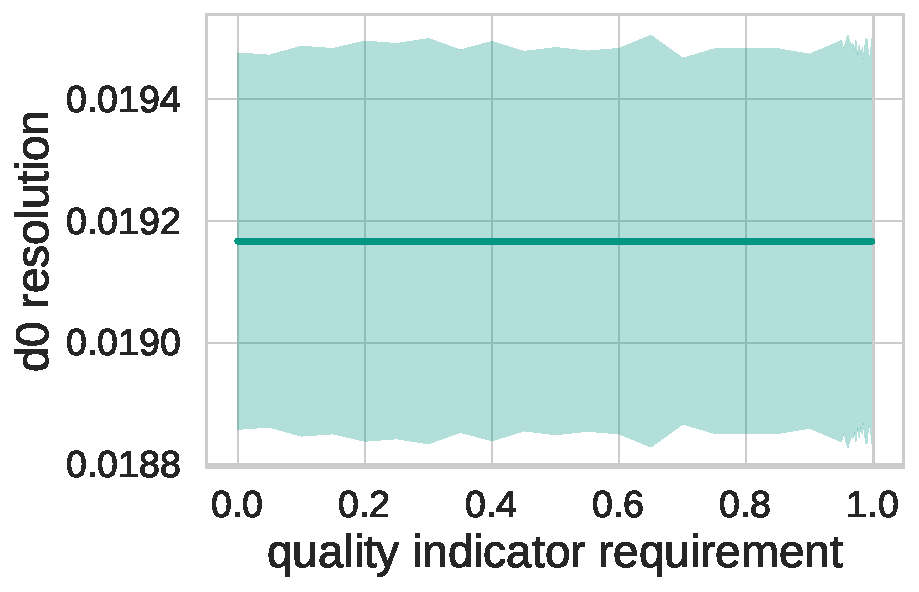
\includegraphics[width=\textwidth]{figures/combined-qi/d0_resolution.pdf}
    \end{column}
    \begin{column}{.33\textwidth}
      \centering
      \includegraphics[width=\textwidth]{figures/combined-qi/z0_resolution.pdf}
    \end{column}
    \begin{column}{.33\textwidth}
      \centering
      \includegraphics[width=\textwidth]{figures/combined-qi/pt_resolution.pdf}
    \end{column}
  \end{columns}
  \begin{columns}
    \begin{column}{.33\textwidth}
      \centering
      \includegraphics[width=\textwidth]{figures/combined-qi/tan_lambda_resolution.pdf}
    \end{column}
    \begin{column}{.33\textwidth}
      \centering
      \includegraphics[width=\textwidth]{figures/combined-qi/phi0_resolution.pdf}
    \end{column}
  \end{columns}
\end{frame}

\end{document}

%%% Local Variables:
%%% coding: utf-8
%%% mode: LaTeX
%%% TeX-engine: default
%%% TeX-master: t
%%% fill-column: 100
%%% ispell-dictionary: "english"
%%% eval: (flyspell-mode 1)
%%% eval: (add-to-list 'TeX-outline-extra '("\\\\frametitle\\b" 7))
%%% End: